\documentclass{sig-alternate}
\usepackage{cite}

\begin{document}

\title{Sense of Community Index, reliability of measurements and their differences among race}
\author{
\alignauthor
Chris Aga \\
\affaddr{ 
University of Minnesota, Morris \\
600 East 4th St. \\
Morris, Minnesota 56267} \\
\email{agaxx010@morris.umn.edu}
}

\date{Today}

\maketitle


%\begin{abstract}
%Abstract.
%\end{abstract}

\keywords{Sense of Community, Sense of Community Index, African Americans, Information response theory, Differential Item Functioning}

\section{Introduction}
Different ethnic groups have differing cultural and historical experiences, because of this it can be difficult to determine if measurement techniques used to gather information between groups are biased towards one group or if they are equal among all groups. This phenomenon is known as differential item functioning (DIF). Psychological sense of community (SOC) is typically measured by sense of community index (SCI) and was analyzed by Coffman for determining if variances were indicative of true racial differences in SOC or if any of the measurements used were biased towards a particular group.

This paper gives a summary of Coffman's experiment and findings in~\cite{disparities:2009} and gives deeper summaries on the approaches used along with reasoning behind mathematical and statistical constructs. The following section gives a background on sense of community, operational constructs and measurement techniques. Section~\ref{sec:experiment} discusses the data-set used for this experiment. Validity of operational constructs for use in SCI is depicted in Section~\ref{sec:dimensionality}. Section~\ref{sec:parameterChoice} then explains calculations made for choosing a proper SCI model. Next, Section~\ref{sec:dif} shows how DIF is statisically tested against the chosen mode, and finally Section~\ref{sec:results} shows the results of the entire experiment.


\section{Sense of Community Background}
\label{sec:background}
Sense of Community (SOC) has various definitions and is extremely important in sociology and psychology. In particular, Sarson introduced SOC in~\cite{sarson:1974} and described it as being one of the most important concepts for definition of self. Sense of Community as defined by McMillan in~\cite{senseOfCommunity:1996} as ``a spirit of belonging together, a feeling that there is an authority structure that can be trusted, an awareness that trade, and mutual benefit come from being together, and a spirit that comes from shared experiences that are preserved as art''. 
\subsection{Operational Constructs}
Varying definitions exist concerning this term, but most literature follows a 4-piece operational system of SOC. The first construct is membership, which describes the idea that when people invest themselves into a community, they have a certain sense of a right to belong~\cite{definition:1986}. Influence, as defined by Peterson as ``a sense that one matters, or can make a difference, in a
community and that the community matters to its members''~\cite{fourFactor:2008}. The third construct, dealing with the idea that the things desired and values shared in a community are similar or are the same. This is termed `reinforcement of needs'~\cite{disparities:2009}. Finally, SOC is also measured in this four-part operational construct system by a `shared emotional connection' between member of the community. 
\paragraph{Validity of four factors}
Many studies have been conducted on these four constructs to determine their relevancy and overall weight in the calculation of an individual's SOC, or Sense of Community Index (SCI). Some have found that these four factors should be measured individually and combined with differing weights to determine one's SCI, while others have found no validity in these measurements and insist that SCI be measured as a one-factor solution. SCI as both a one-factor and four-factor instrument was heavily studied by Chipuer in ~\cite{oneFactor:1999}. The one-factor approach was determined as valid, and the four-factor approach had validity but there was much less consistency of measurements between data-sets than with the one-factor approach.


\section{Experiment}
\label{sec:experiment}
Coffman in~\cite{disparities:2009} attempted to determine if SCI differences were attributable to true differences in the amount of SOC between blacks and whites or if any of the questions used to calculate the SCI values were nonequivalent measures between race. This concept is known as differential item functioning, and concerns the prevention of biases of a certain measurement when looking at exogenous variables such as gender sex or race. 

\subsection{Data}
The data-set used for Coffman's experiment consisted of 1,463 interviews to determine SCI. The interviews were conducted ``using computer assisted telephone interview (CATI) technology''~\cite{disparities:2009}. The entire data-set used consisted of 588 whites and 840 blacks and a total of 12 questions were asked to determine an individual's SCI. The questions were yes/no and thus the overall score ranged from 0-12 with higher numbers indicating a stronger perceived SOC. 

\section{Dimensionality}
\label{sec:dimensionality}
\subsection{Overview}
Before undergoing the main experiment, Coffman determined the number of factors from the four SOC operational constructs to be used. The final number of factors was carefully determined by a mathematically rigorous process known as full information factor analysis. 
\begin{figure*}
\centering
\label{fig:questions}
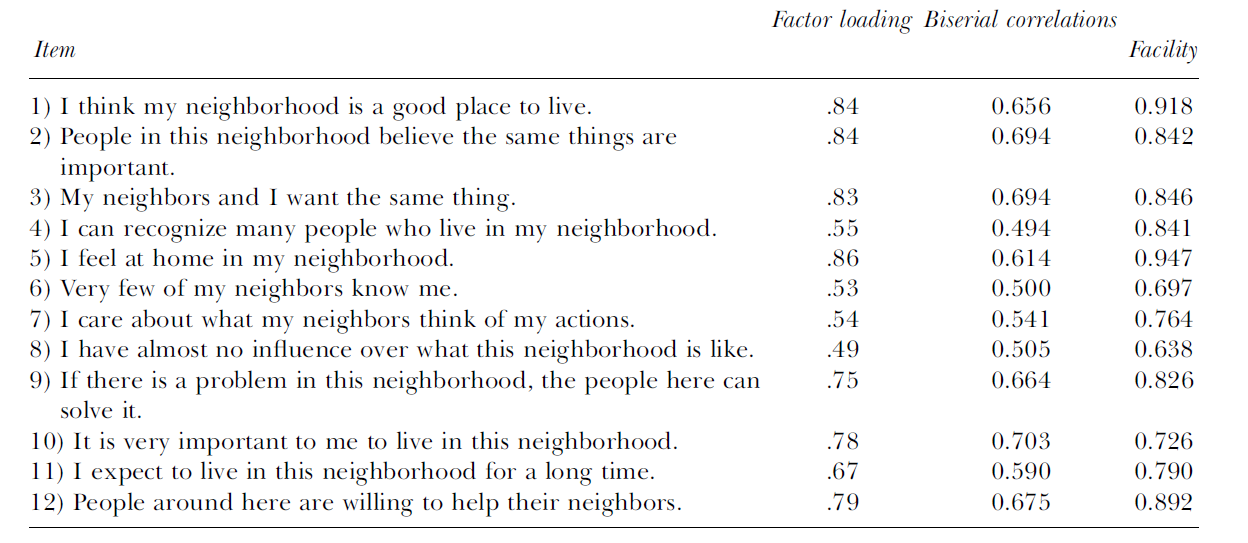
\includegraphics[scale=0.5]{Images/questions.png}
\caption{Table of questions used to determine SCI, includes factor loadings which describe the weight of each question when determining SCI and analyzing DIF~\cite{disparities:2009}}
\end{figure*}

\subsection{Computation and explanation}
Full information item factor analysis first involved calculating the probability of a $person_i$ with a SOC score of $\theta$ answering yes to a particular $question_j$. SOC score in the one-factor model is $\theta$, whereas in for example, a four-factor model (all four operational constructs for sense of community) is represented as scores in: \\$\theta = (membership, influence, similarity, reciprocity)$.\\ Probability is a function of item facility (the number of people who answered yes to a question), standard deviation in answers to a question and the mean answers to a question. 

A probability distribution is generated for the entire data-set and is then integrated over to determine the probability of answering $question_j$ with a certain response. A core factor in the score is using what is known as ``factor loading''. Factor loading is a weight applied to each operational construct for SOC, and these factors are calculated by minimizing the error output of the model. The combination of factor loadings and a person's ability are combined in the probability function as described by Equation~\ref{eq:ability}.
\begin{equation}
\label{eq:ability}
ability = \sum\limits_{k = 1}^{m} \alpha_{jk} \theta_{ki}
\end{equation}

Marginal probability is then computed for $question_j$ based on all the probabilities per person with each specific vector of SOC factor scores. Finally, this marginal probability is combined along with a null hypothesis (not explained at all by the author for this particular experiment) and then a goodness-of-fit test (g-test) is applied. Initially one factor is used, full information analysis is computed, then g-test is applied. If the output is not statistically significant, no further factors are added and the dimensionality is now known for the SCI model~\cite{analysis:1988}.

\section{Choice of parameters logistic model}
\label{sec:parameterChoice}
\subsection{Models}
After assessing proper dimensionality for the experiment, a proper item response theory model must be chosen to determine which parameters are applicable to each question for studying this data-set. The parameters include difficulty and discrimination. Difficulty in this experiment was the standard deviation from average SOC within a group, of a person having a 50\% chance to answer yes to a question~\cite{disparities:2009}. Discrimination describes 


The second parameter is discrimination, which as defined by Baker in~\cite{irt:2001}, ``describes how well an item can differentiate between examinees having abilities below the item location and those having abilities above the item location.'' Discrimination was calculated using factor loadings which were based off of standard deviation in responses.

Many times a third, `guessing' parameter is used since IRT often is used for knowledge assessment to prevent persons with lesser knowledge from simply achieving a higher score though lucky guessing. This however was not included in Coffman's experiment since most people will not have to resort to guessing to answer questions such as ``I care about what my neighbors think of my actions''.

\subsection{Statistical analysis for final choice}
\label{sec:irtModel}
Three models were suggested and tested to determine the proper approach for this experiment. Two 1PL models, one with a discrimination of 1 for each question, the other with an estimated discrimination value (equivalent for each question), and a 2PL model with discrimination values determined by factors loadings. The model used was chosen by comparing ``Akaike information criterion, and Bayesian information criterion and log-likelihood nested tests'' for each approach~\cite{disparities:2009}.



\section{Differential Item Functioning}
\label{sec:dif}
Once all of the setup is completed, the core component of this experiment can be evaluated. In particular, Coffman wanted to assure that all questions being used to evaluate an individual's SOC were not biased towards a particular group. After parameter value(s) (depending on 1PL or 2PL model) are gathered for each question, differential item functioning (DIF) is applied to each parameter to see if they are variant from group to group. The null hypothesis used for this experiment will be discussed later seeing as they are dependent on the chosen IRT model.

\subsection{Calculation of Differential Item Functioning}
Swaminathan in~\cite{logisticDIF:1990} describes various approaches to calculating the DIF of items of single or multiple factors as well as working with models made up of single or multiple parameters for characteristics of questions. As will be depicted in Sections~\ref{sec:dimensionality} and~\ref{sec:parameterChoice}, a one-factor, two-parameter based model was chosen and thus the following procedure for calculating DIF was used. 

First, a predictor for probability of answering yes to a question by modeling between different groups is described by Equation~\ref{eq:probabilityLogistic}. The difficulty of a question is $\beta_{0j}$, variance of response on an item for people with the same SOC score is represented by $\beta_{1j}$, and $\theta_{ij}$ describes the SOC of $person_i$ in $group_j$.
\begin{equation}
\label{eq:probabilityLogistic}
P =  \frac{e^{(\beta_{0j} + \beta_{1j}*\theta_{ij})}}{1+e^{(\beta_{0j} + \beta_{1j}*\theta_{ij})}} 
\end{equation}

Swaminathan defines DIF as: ``an item shows DIF if individuals with the same ability but from different groups do not have the same probability of success on the item''~\cite{logisticDIF:1990}.
Coffman explains that these probabilities between groups are transformed into chi-squared distributions then statistically analyzed to determine if any of the parameters demonstrate DIF within the experiment~\cite{disparities:2009}.



\section{Results}
\label{sec:results}
\subsection{Chosen dimensionality}
Full information item factor analysis was conducted on the gathered data-set multiple times to determine the proper dimensionality to use for this experiment. Though statistical analysis in TESTFACT, a program for scoring tests, and calculating factor analysis. The results, due to loss of significance in g-tests showed that a one-factor model was to be used for the experiment instead of using multiple operational constructs for scoring of SOC. Factor loadings for each question were generated from the one-factor full-information-analysis and are shown in~\ref{fig:questions}.
\begin{figure*}
\label{fig:probability}
\begin{center}$
\begin{array}{cc}
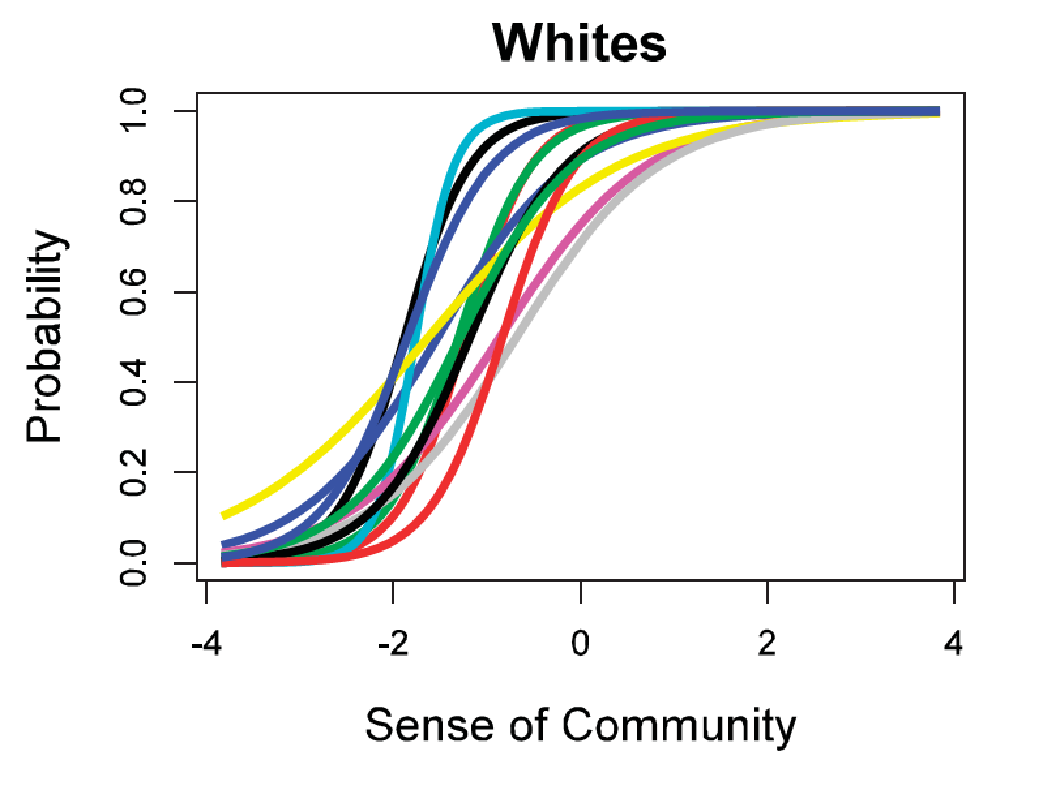
\includegraphics[width=2.5in, height=2in]{Images/whiteProb} &
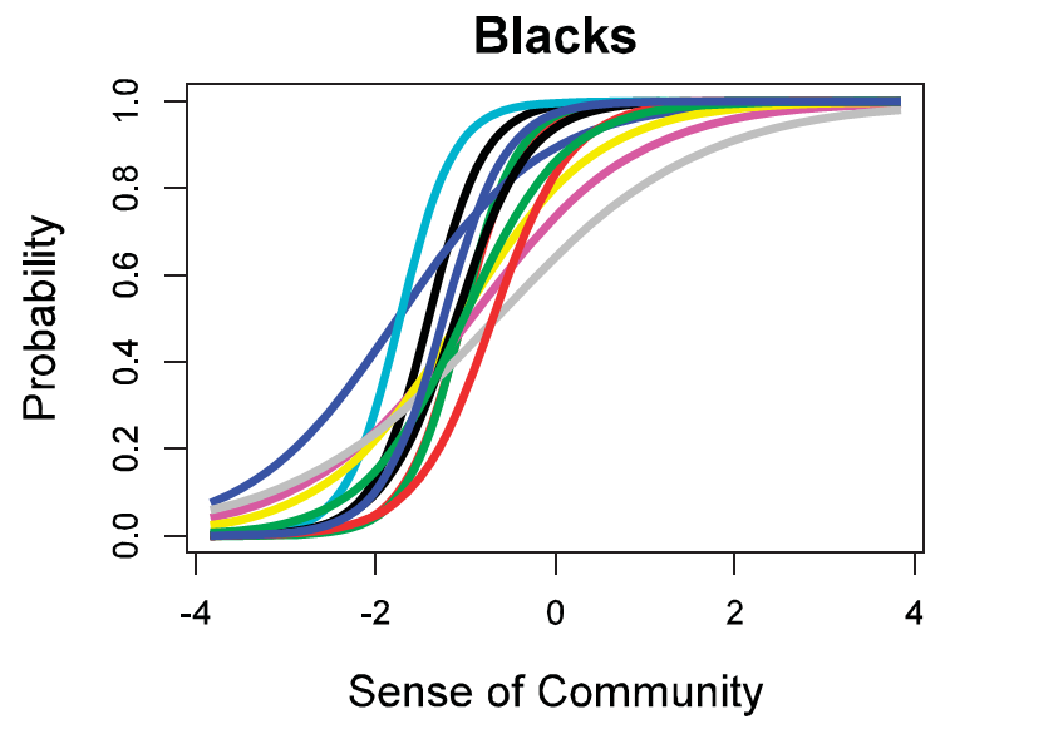
\includegraphics[width=2.5in, height=2in]{Images/blackProb} \\ 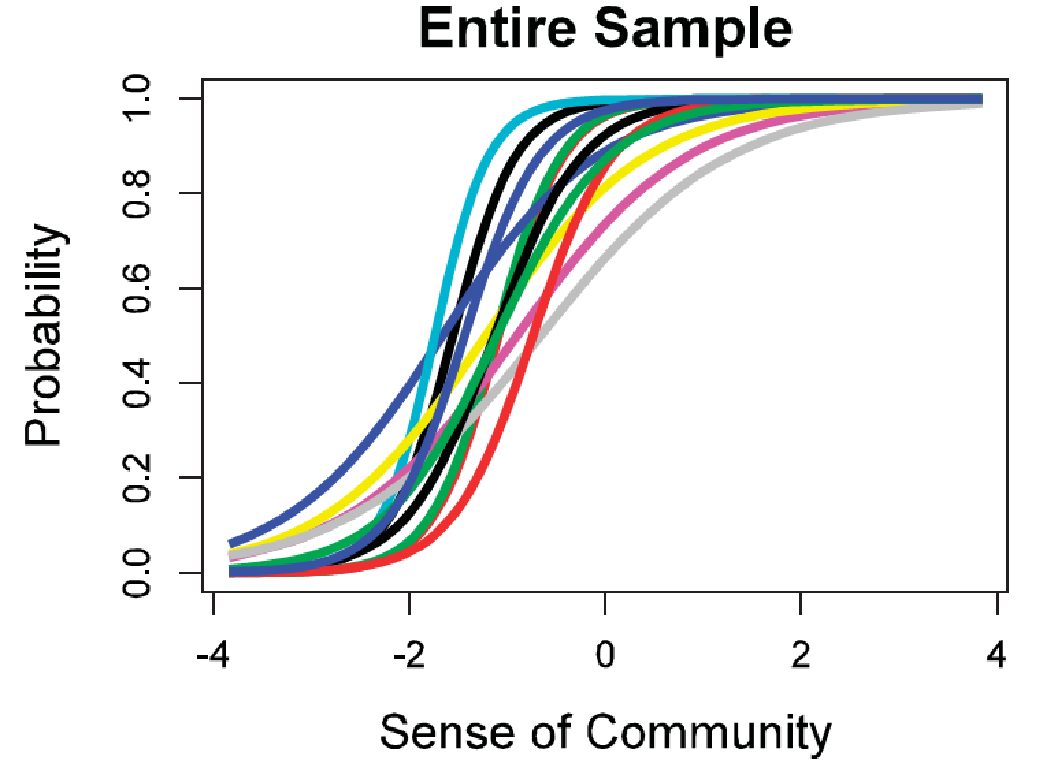
\includegraphics[width=2.5in, height=2in]{Images/allProb}
\end{array}$
\end{center}
\caption{Probability distribution of all 12 questions for whites blacks and for all candidates}
\end{figure*}
Biserial correlations were a coefficient that described the relationship between a question and the average SOC of a group or groups. A large biserial correlation for a question would mean that people who got high SOC scores typically answered yes to this question. Facility was the percentage of people in the entire data-set who answered yes to a particular question~\cite{biserial:2006}.

\subsection{Choice of information response theory model}
The statistical analysis tool R was used, and a latent trait modeling (LTM) package was implemented to determine the proper IRT model for this experiment. The three statistics described briefly in Section~\ref{sec:irtModel} were calculated by LTM, compared for significance and the chosen model was 2PL. Thus both difficulty and discrimination parameters were included and examined for statistically significant DIF~\cite{disparities:2009}.

\subsection{Differential item functioning analysis}
Probability distributions were generated for each item, for both blacks, whites and a combination of both groups to illustrate the overall impact each question had based on scored SOC. These results are shown in Figure~\ref{fig:probability}.


Information plots were also generated for the means of determining if particular items were more accurate descriptors of SOC for blacks or whites. Information in IRT, as described by Baker, is calculated using the precision of an item's parameter. Baker in~\cite{irt:2001} uses Equation~\ref{eq:variance} to produce information I. $\sigma$ represents the amount of standard deviation, this value is squared to get variance, then the reciprocal is computed to obtain I.
\begin{equation}
\label{eq:variance}
I =  \frac{1}{  \sigma ^{2} } 
\end{equation}
Standard deviation in~\cite{disparities:2009} is described by how much the SOC value varies from a probability of 0 to 1. Therefore, questions will low standard deviations will, based on Equation~\ref{eq:variance}, depict how useful a question is at determining someone's SOC. 

If information differences at the same value of SOC are statistically significant then DIF is computed to determine if a $question_x$ is a good indicator at determining SOC differences between race or if $question_x$ is not important for the actual determination of SOC~\cite{disparities:2009}.
Significant differences in a particular question, ``I feel at home in my neighborhood'' were found at areas of similar SOC between blacks and whites in the experiment, thus DIF was calculated on the results to determine how accurate of a determiner this question was for each group. After statistically analyzing parameters for DIF, none were found.

\section{Discussion}
\label{sec:discussion}
Full information factor analysis found that a one-factor approach (amount of SOC versus SOC calculated from amounts of membership etc) was a correct dimensionality to use for SCI in this experiment. Coffman described how other research found support for four-factor SCI models, but explained that differences in those studies versus this study demeaned assurance of accurate models. First, data was dichotomous since the questions asked were either yes or no, thus full information factor analysis for choosing proper dimensions was necessary~\cite{disparities:2009}. Also, other studies such as~\cite{validation:2008} had used different scales for measuring SOC, thus their finding of four-factor support were not valid for justifying its automatic acceptance in this experiment. 

After all the appropriate models were chosen, DIF was calculated for both difficulty and discrimination parameters on each question. Greater information was found for one question (5) when determining SOC for whites as opposed to blacks. But after statistical analysis on both question parameters, DIF was no existent thus differences in SCI between blacks and whites were likely indicative of true differences in SOC between race. 

For question 5, ``I feel at home in my neighborhood'', low standard deviation was found in particular or white, so it mean that this was a good indicator for measuring a white person's SOC because of more consistent answers at particular SOC scores. But, white people with SOC score $\theta$ did not tend to answer yes much more than black people with the same $\theta$ score, they just had more consistent answers to this question. These results show that differences in SCI measurements between blacks and whites are not attributable to differential item functioning in a particular question, but are more likely measures of true race differences in SOC. 

\nocite{*}

\bibliography{Bibliography}
\bibliographystyle{abbrv}
\end{document}